\section{System's Perspective}


\subsection{Design and Architecture}
% \textcolor{red}{Design and architecture of your ITU-MiniTwit systems.}

Our ITU-MiniTwit systems consists of a web service and an API service, both written in Golang, which act in a client-server architecture. Data is stored in a PostgreSQL database. 

\red{Her kommer der et fucking diagram}

The UML deployment diagram in figure \ref{fig:deployment} shows how the different components in our system is deployed. All technologies and components are described in detail in the following section.

\begin{figure}[H]
    \centering
    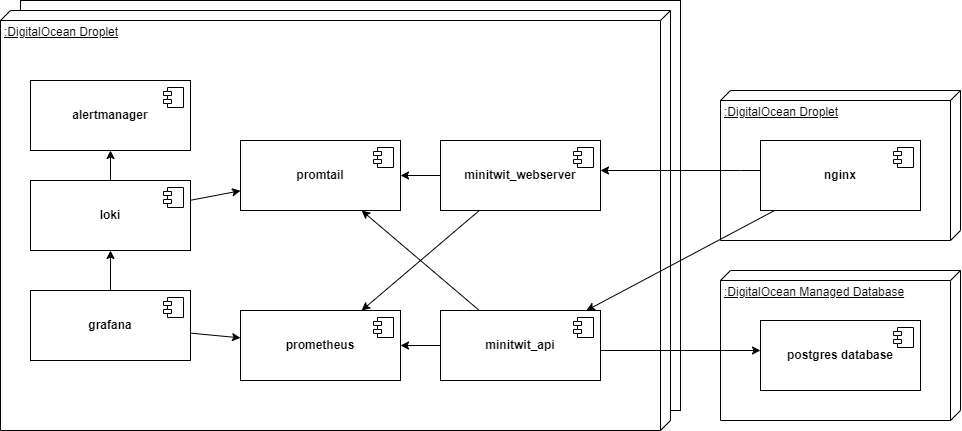
\includegraphics[width=0.8\textwidth]{images/deployment.png}
    \caption{UML Deployment Diagram}
    \label{fig:deployment}
\end{figure}


\subsection{Technologies and tools}
%\textcolor{red}{ All dependencies of your ITU-MiniTwit systems on all levels of abstraction and development stages. That is, list and briefly describe all technologies and tools you applied and depend on.}
This sections provide a overview and description of the technologies and tools utilized throughout our project work.


\subsubsection*{List of Technologies and Tools Utilized}

\begin{multicols}{2}
    \begin{itemize}
        \item \textbf{Go}: A statically typed, compiled programming often used for backend development.
        \item \textbf{Go/Gorilla}: A toolkit for Golang, that provides packages for building web applications. Used for routing and session management.
        \item \textbf{SQLite}: A lightweight SQL database engine that is ideal for embedded database applications. Used in initial setup and for testing.
        \item \textbf{Docker}: A platform for shipping and running applications, ensuring consistency across different environments. Containerization is used deliberately throughout our system and in delivery.
        \item \textbf{Docker Swarm}: A container orchestration tool, included in Docker by default, to manage a cluster of Docker nodes as a single virtual system.
        \item \textbf{DigitalOcean}: A cloud infrastructure provider offering scalable compute and storage solutions. Used for deploying and managing the application and database.
        \item \textbf{Prometheus}: An open-source monitoring toolkit used for monitoring metrics in our cloud environments.
        \item \textbf{Grafana}: An open-source analytics and monitoring platform that integrates various data sources to visualize our data and metrics.
        \item \textbf{PostgreSQL}: A open-source object-relational database system, known for extensibility and speed. Used after the transition from SQLite managed by DigitalOcean.
        \item \textbf{Promtail}: An agent that ships log file to Loki and part of the Grafana logging stack. Used for gathering logs.
        \item \textbf{Loki}: A log aggregation system designed to be scalable. Used with Grafana for log querying and visualization.
        \item \textbf{Nginx}: A high-performance web server and reverse proxy server. Used for load balancing.
        \item \textbf{CertBot}: A open-source tool for automatically using Let's Encrypt certificates to enable HTTPS on web servers.
        \item \textbf{Terraform}: An infrastrcucture as code tool that allows users to define and provision data center infrastructure using a high-level configuration language. 
    \end{itemize}
\end{multicols}

\subsubsection*{Technology choices}%should maybe just be in text when relevant

% \red{MSc should argue for the choice of technologies and decisions for at least all cases for which we asked you to do so in the tasks at the end of each session.}

Our initial choice of language for refactoring ITU-MiniTwit was based on a detailed feature mapping of the system and a comparison of programming languages (see Appendix \ref{app:programming_language_choice}). 

This analysis led us to initially select Crystal/Kemal. However, we soon discovered that Kemal's documentation was insufficient, making it challenging to work with. Consequently, we switched to Golang, which offered similar features but had much more comprehensive documentation.





\subsection{Subsystem interactions}

% \red{Important interactions of subsystems.
% For example, via an illustrative UML Sequence diagram that shows the flow of information through your system from user request in the browser, over all subsystems, hitting the database, and a response that is returned to the user.
% Similarly, another illustrative sequence diagram that shows how requests from the simulator traverse your system.}

Figure \ref{fig:user_sequence} shows the flow of information seen from the perspective of a user accessing the website. Initially the user reaches the load balancer, nginx, connecting and forwarding the request to one of the webserver replicas that then looks back to nginx with a request for a backend api. When the backend receives the request it sends the query for recent messages to the database as well as logs and updates monitoring metrics before returning the response to nginx and then to the webserver. Ultimately the webserver serves the final page to the user through nginx using the messages receives from the backend.


\begin{figure}[H]
    \centering
    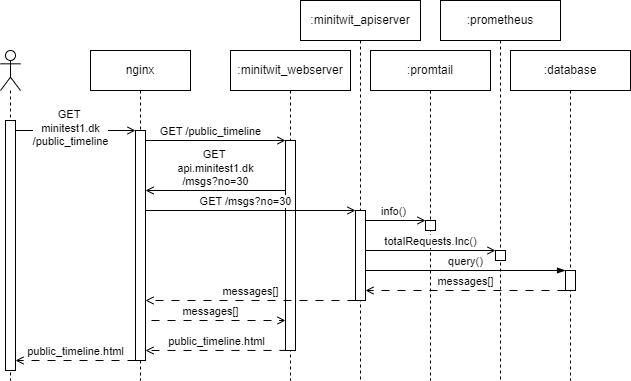
\includegraphics[width=0.8\textwidth]{images/sequence.png}
    \caption{Sequence diagram of the user interacting with the system.}
    \label{fig:user_sequence}
\end{figure}

The simulator interaction is very similar to the interaction of the user except for the fact that it does not need to go through the webserver. The flow of a POST request can be seen in the sequence diagram in figure \ref{fig:sim_sequence}. One thing to note is that we have not been stress testing the user perspective in this course as all requests have come from the simulator. This means that we do not have data to reflect on the performance of our nginx setup which results in a lot of back and forth messaging as seen in the first diagram. 

\begin{figure}[H]
    \centering
    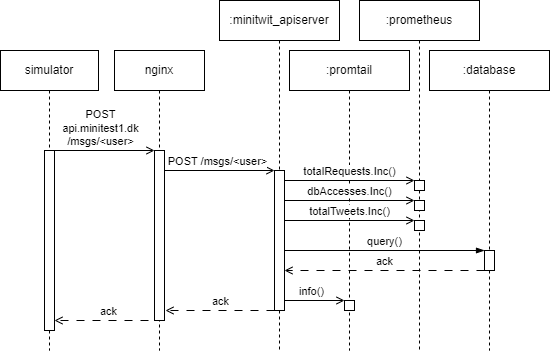
\includegraphics[width=0.8\textwidth]{images/sequence-simulator.png}
    \caption{Sequence diagram of the simulator interacting with the system.}
    \label{fig:sim_sequence}
\end{figure}




\subsection{Current state}
%\textcolor{red}{Describe the current state of your systems, for example using results of static analysis and quality assessments.}

At the time of writing, our ITU-MiniTwit system is being evaluated using the static code analysis tools, Code Climate and SonarCloud.
For an overview, see Appendix \ref{app:static_analysis}. In summary, both tools reveal that while the system has a good level of maintainability and security, the following areas require improvement:

\begin{itemize}
    \item \textbf{Code Smells}: Identified in Code Climate, these primarily consist of functions with an excessive length and functions with multiple return statements. 
    \item \textbf{Duplications}: Identified in SonarCloud, we exceed the suggested amount of duplicated code. This is primarily duplicated code blocks between our API and the front-end, related to database connections.  
    \item \textbf{Test Coverage}: Implementing and configuring comprehensive test coverage to accurately reflect this metric in both Code Climate and SonarCloud.
    \item \textbf{Maintainability issues}: The specific issues noted in SonarCloud should be resolved according to their estimated effort to maintain and ensure a low technical debt ratio.
\end{itemize}

Addressing these areas will improve the current state of our codebase and ensure long-term maintainability. 
\textcolor{red}{Den siger current state, men jeg har skrevet noget der siger lidt om hvordan vi har brugt de tools, fjern hvis ikke fedt}
During the project we have however listened to the feedback from these tools and made changes. 
In one instance we refactored our api and src directories from being a single python file to many different files based on their responsibilities resulting in an easier overview of the code base and increasing maintainability.
